\section{Couette flow with chain molecules}
The next task was to simulate a Couette flow system with two walls moving in opposite directions at velocity $v_{wall} = 5$. Furthermore the system contained $42$ chain molecules, which are structured as $A-A-B-B-B-B-B$, and fluid particles. Bond parameters wereg given as $K_S = 100$ and $r_S = 0.1$, in addition conservative force coefficients were set according to the matrix given in the assignment.
\begin{figure}[H]
	\begin{center}
		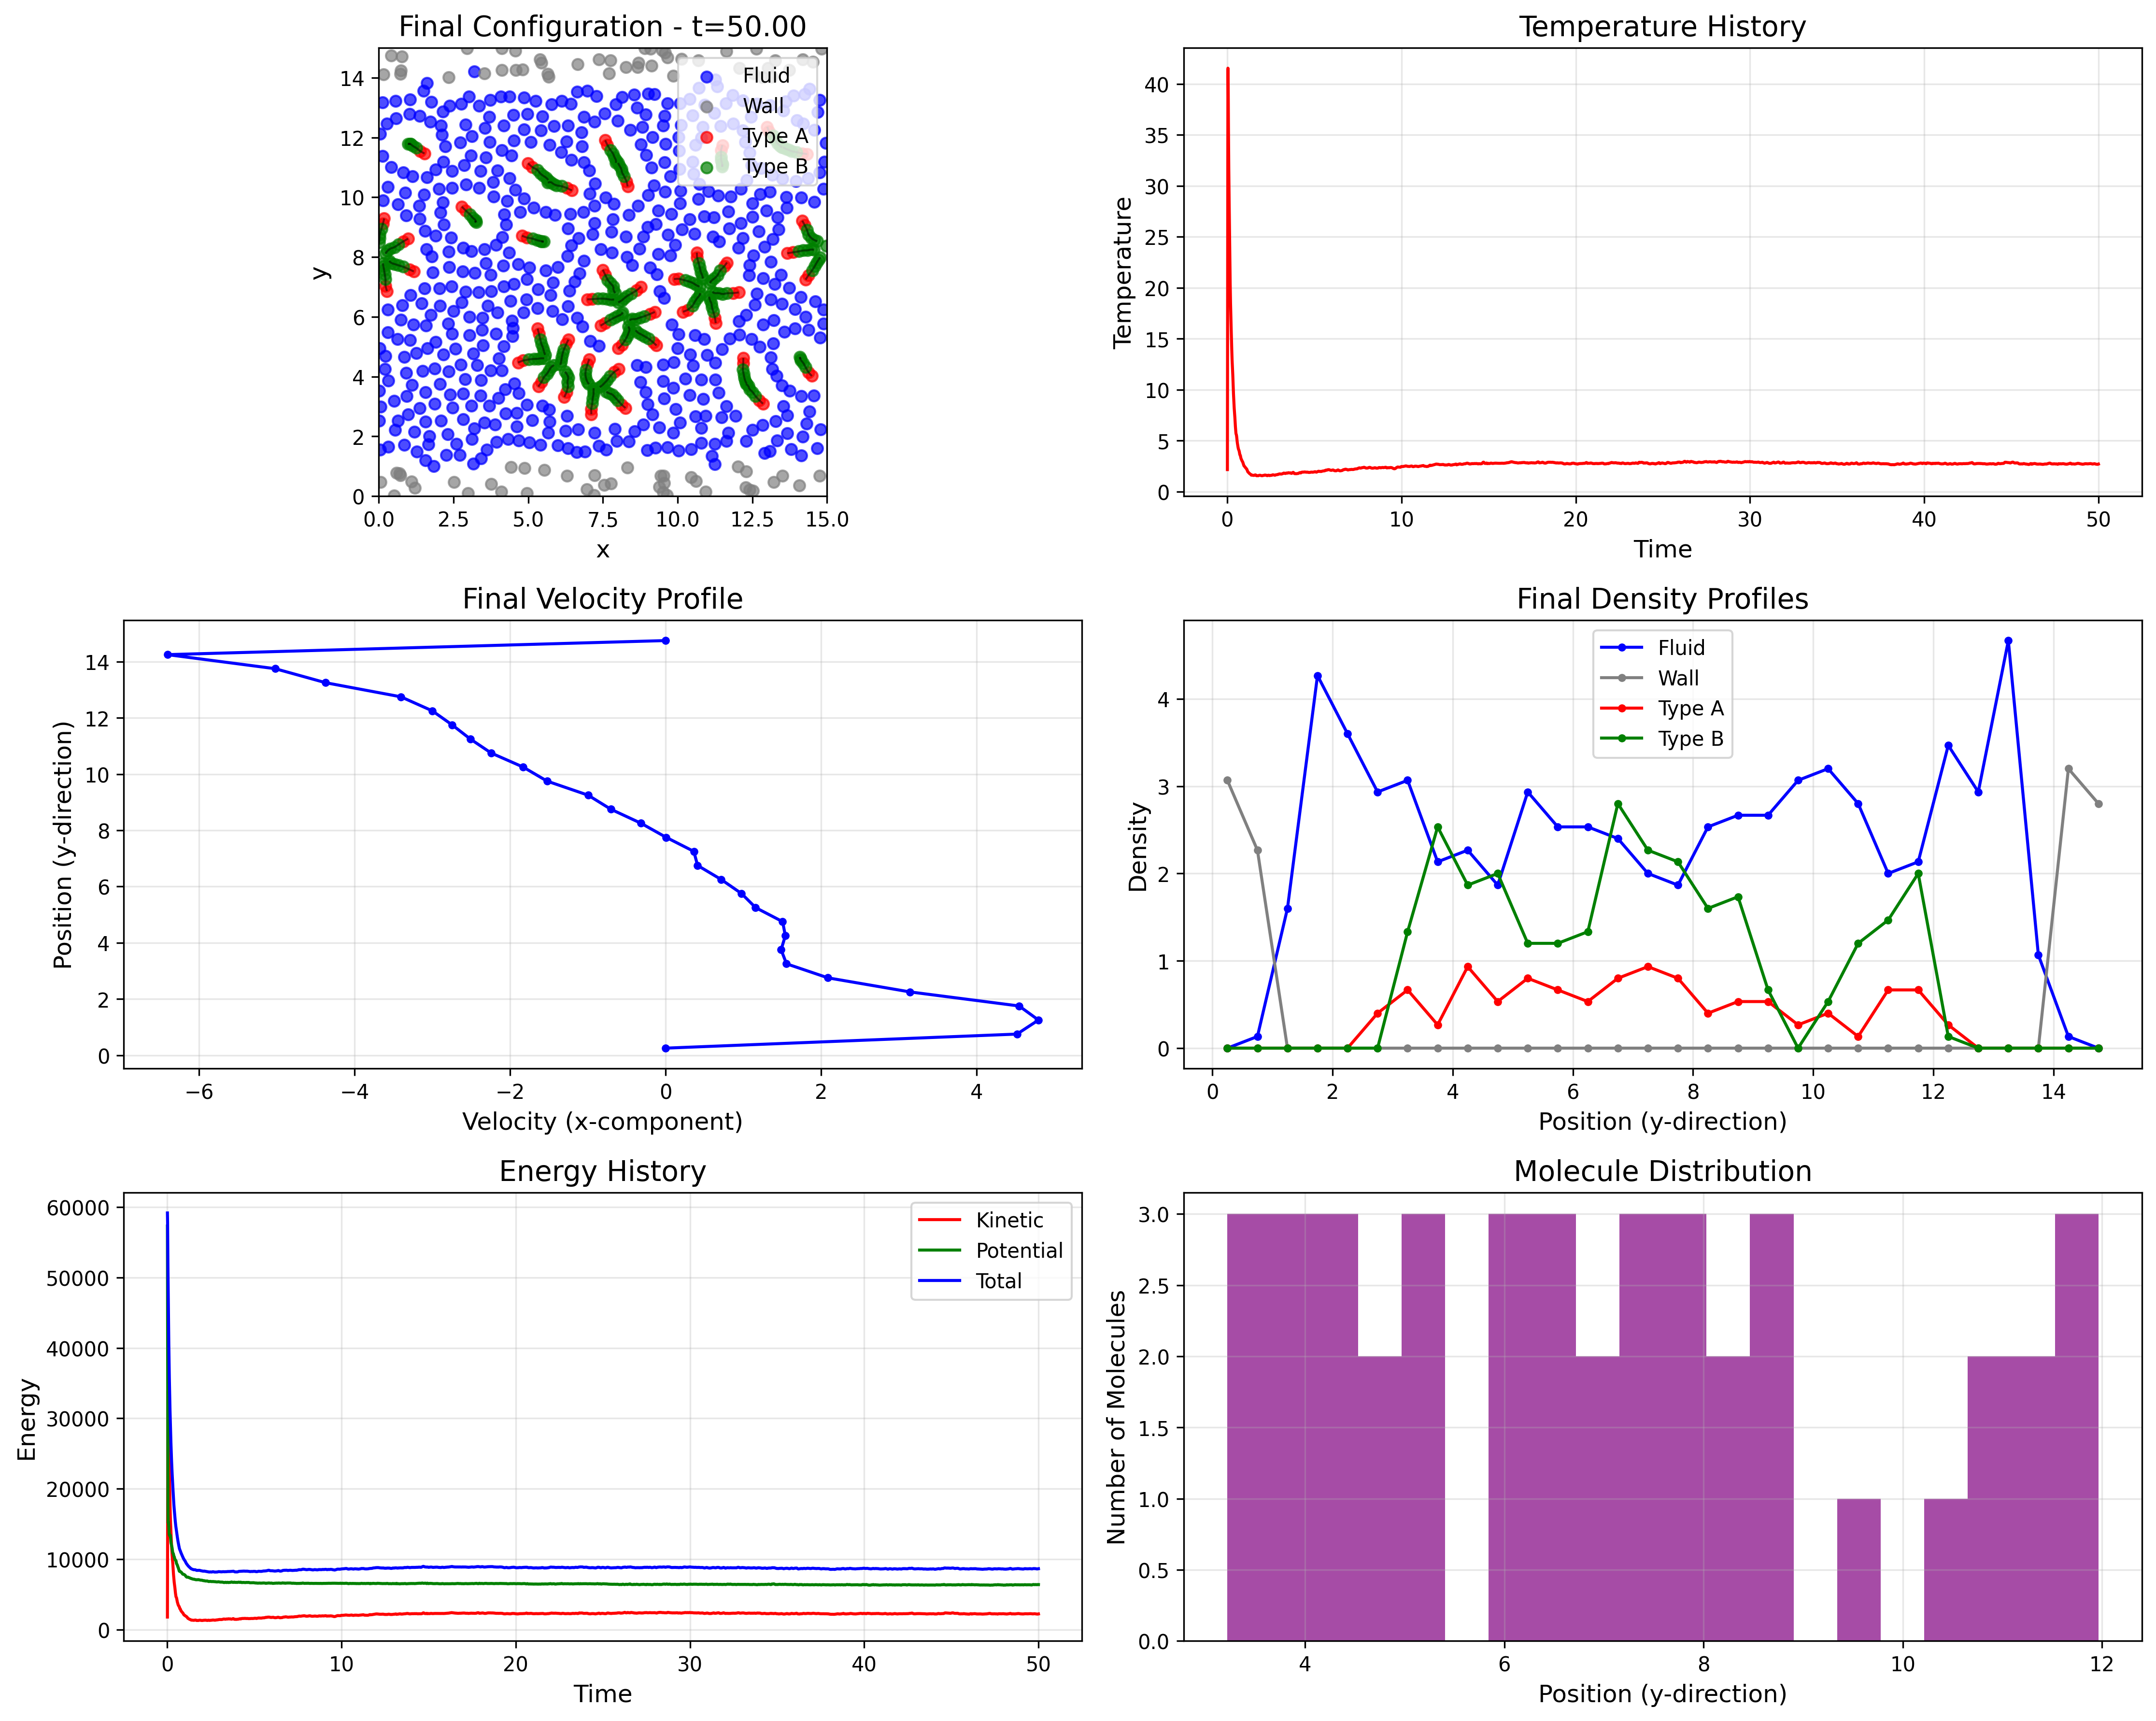
\includegraphics[width=0.95\textwidth]{figures/couette_final_vis.png}
	\end{center}
	\caption{Couette flow with $dt = 0.01$ and $5000$ steps.}\label{fig:couette}
\end{figure}
\subsection{Flow Profile Analysis}
Figure \ref{fig:couette} shows that after $5000$ timesteps, the velocity profile demonstrates a nearly linear relationship between position and velocity in the central region, which is an expected characteristic of Couette flow. Near the walls, there are some deviations from linearity due to the discrete nature of the walls and molecular interactions.
\subsection{Molecule Distribution and Motion}
We can observe several interesting behaviors of the chain molecules during the simulation:
\begin{enumerate}
	\item The molecules tend to align with the flow direction due to shear forces.
	\item There is a noticeable depletion of chain molecules near the walls and some concentration in the center region.
	\item The distribution of molecules is not completely uniform across the channel.
\end{enumerate}
This behavior can be explained by the interactions. The repulsion between type B and fluid particles ($a_{BF} = 300$) leads to the ends which have B particles to avoid fluid-dense regions. Additionally, the weak interaction between B-B particles ($a_{BB} = 1$) leads to them  approaching each other rather closely, leading to aggregation of the chains. The walls on the other hand repel all particle types ($a_{iW} = 200$), creating a "depletion layer" near the boundaries.
The molecules are rotating as they move through the flow, with the shear forces causing them to tumble. This rotation is more noticeable in the center of the channel where the velocity gradient is the highest.
